\section{Models}
\label{sec:method}

We design a machine learning model that predicts assistant and user actions.
We introduce a multi-task architecture for \textbf{C}uriosity that \textbf{H}ier\textbf{ar}chically \textbf{M}odels (\charm{}, Figure~\ref{fig:model}) dialogs to:
(1) predict the dialog acts of the user message~(utterance act prediction),
(2) select the best fact~(fact prediction),
(3) choose the best set of dialog acts for the next message~(policy act prediction),
and (4) predict if the assistant message will be liked~(like prediction).

\begin{figure*}[t]
    \centering
    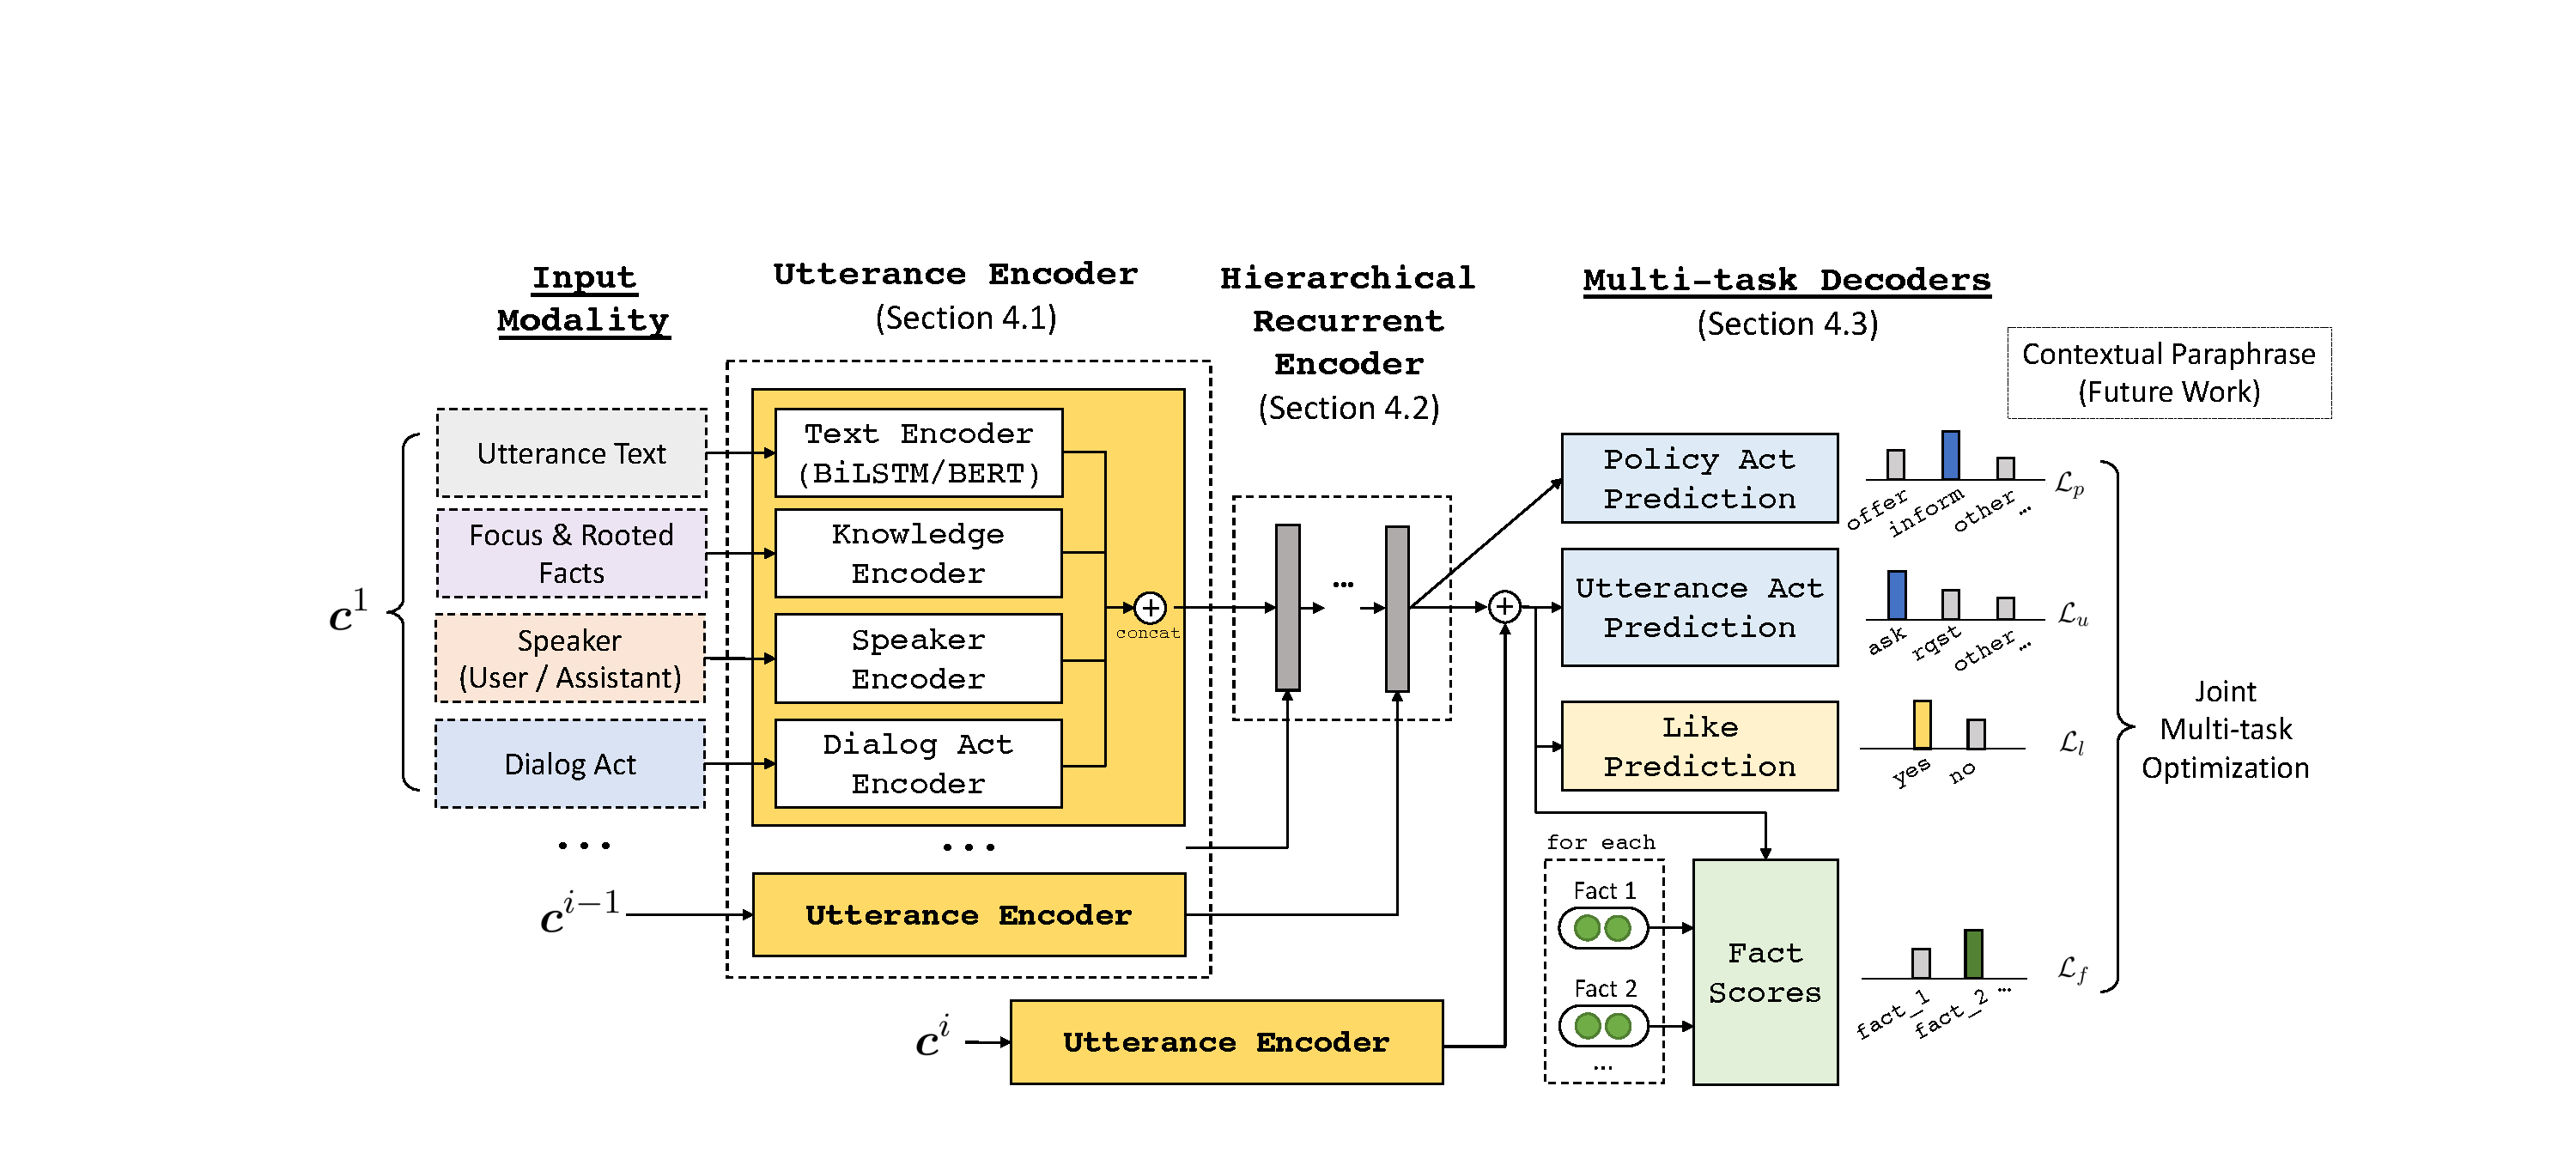
\includegraphics[width=\linewidth]{2020_emnlp_curiosity/figures/charm-model}
    \caption{
        \textbf{Architecture}: \abr{charm} builds a dialog context up to $t=i-1$ to predict the current message's dialog acts~(policy prediction) and the best facts to use.
        The model uses this combined with the current utterance to classify it's dialog acts and if it will be liked.
    }
    \label{fig:model}
\end{figure*}

\subsection{Text Representation}
\label{subsec:method:text}
\charm{} jointly encodes the text of utterances and facts with one encoder.
$E$ is a bi-directional \abr{lstm}~\citep{Sutskever2014SequenceTS} over \glove{}~\citep{pennington2014glove} word embeddings and Wikipedia2Vec~\citep{yamada2018wikipedia2vec} entity embeddings.\footnote{
    In \charm{}, \bert{} was not as effective an encoder.
}
The text $t_i^u$ of utterance $u_i$ in dialog $D$ is represented as $E(t_i^u$).
Similarly, fact~$f_j$ on turn~$i$ is represented as $E(t_{i,j}^f)$ where~$j$ indexes facts shown on that turn.

\subsection{Dialog Representation}
\label{subsec:method:dialog}
In our models, we use a hierarchical recurrent encoder (\hre{}) architecture~\citep{Sordoni2015AHR,Serban2015BuildingED} where a forward \abr{lstm} contextualizes each utterance to the full dialog.
We modify the \abr{hre} model by adding additional inputs beyond the utterance's textual representation.
First, we represent user's known entities
\begin{equation}
    \bm{k}=\text{avg}(E_{\text{entity}}(e_1),\ldots,E_{\text{entity}}(e_k)))
\end{equation}
as the average of entity embeddings.
An entity embedding also represents the topic
\begin{equation}
    \bm{t}=E_{\text{entity}}(\text{topic)}
\end{equation}
of the dialog.
Next, we create trained speaker embedding $\bm{v}_s$ for the user and $\bm{v}_t$ for the assistant.
Given the set of all dialog acts $\mathcal{A}$, each utterance has a set of dialog acts $\mathcal{A}_u\in\mathcal{P}(\mathcal{A})$ where $\mathcal{P(X)}$ denotes the set of all subsets of $\mathcal{X}$.
Finally, we use an act embedder $A$ to compute an act representation
\begin{equation}
    \bm{a}^i=\frac{1}{|\mathcal{A}_u|}\sum_{a_k\in\mathcal{A}_u} A(a_k)
\end{equation}
by averaging embeddings at each turn.
The input at each step is the concatenation
\begin{equation}
    \bm{c}^i=[E(t_i^u);\bm{a}^i;\bm{t};\bm{k};\bm{v}]
\end{equation}
of the representations for text, speaker, topic, known entities, and utterance dialog acts.\footnote{
    The speaker embedding $\bm{v}$ alternates between $\bm{v}_s$ and $\bm{v}_t$.
}
With this joint representation, the contextualized dialog representation
\begin{equation}
    \bm{h}^{i-1}=\text{LSTM}(\bm{c}^1,\ldots,\bm{c}^{i-1})
\end{equation}
is the final \abr{lstm} state and includes time step~$t=i-1$.
The dialog up to and including time $i$ is
\begin{equation}
    \bm{d}^i=[\bm{h^}{i-1};\bm{c}^{i}]
\end{equation}
which emphasizes the current utterance and makes multi-task training straightforward to implement.

\subsection{Tasks and Loss Functions}
\label{subsec:method:task}
In our model, we jointly learn to predict fact usage, user likes, utterance acts, and policy acts.
\paragraph{Fact Prediction}
For every assistant turn, the model predicts which fact(s) from
$$\{f_1,\ldots,f_k\}\in \mathcal{F}^{(i)},\mathcal{F}^{(i)}\in\mathcal{P}(\mathcal{F})$$
the assistant marked as ``used'' where $\mathcal{F}$ is the set of all facts.
We frame this task as pointwise learning to rank~\citep{Li2008LearningTR}.
A fact prediction network
\begin{equation}
    \bm{s}_{j}^{f,(i)}=\text{GELU}\left(\left[\bm{W}^f\cdot \bm{h}^{(i-1)} +\bm{b}^f;E(t_j^f)\right]\right)
\end{equation}
with parameters $\bm{W}^f$ and $\bm{b}^f$ using a Gaussian Error Linear Unit~\citep{Hendrycks2017BridgingNA} outputs salience scores for each fact.
The network does not use utterance $u_i$ since it contains signal from the choice of fact.
The predictions
\begin{equation}
    \bm{\hat{y}}^{f,(i)}_j=\text{softmax}(\bm{s}_{j}^{f,(i)})
\end{equation}
are converted to probabilities by the softmax
\begin{equation}
    \text{softmax}(\bm{q})=\frac{exp(\bm{q})}{\sum_{j=1}^k exp({\bm{q}_j})}
\end{equation}
over $k$ labels. Using this, we compute the fact loss
\begin{equation}
    \mathcal{L}_f=\frac{1}{|\mathcal{F}^{(i)}|}\sum_{i,j} \ell_{ce}(\bm{\hat{y}}^f_{i,j},\bm{y}_{i,j})
\end{equation}
where labels $\bm{y}^{f,(i)}_{j}$ indicate if fact from utterance $i$ in position $j$ was used and
\begin{equation}
    \ell_{ce}(\bm{\hat{y}},\bm{y})=\sum_{p=1}^k\bm{y}_p\log(\bm{\hat{y}}_p).
\end{equation}
is the cross entropy loss.
To mitigate class imbalance, we also scale positive classes by nine~\citep{Japkowicz2002TheCI}.

\paragraph{Policy Act and Utterance Act Prediction}
Each utterance may have multiple dialog acts so we treat policy and utterance act prediction as a multi-label task.
The goal of policy prediction is to choose the best act for the next utterance; the utterance act classifies the last message's acts.
To predict these acts, we create a policy act network
\begin{equation}
    \bm{s}^{p,(i)} = \text{GELU}(\bm{W}^p\cdot \bm{h}^{i-1} + \bm{b}^p)
\end{equation}
and an utterance act network
\begin{equation}
    \bm{s}^{u,(i)} = \text{GELU}(\bm{W}^u\cdot \bm{d}^i + \bm{b}^u)
\end{equation}
where the probability of act $a_k$ is $p^{*,i}_k=exp(\bm{s}^{*,(i)}_k)$.
From these, we derive the policy act loss
\begin{equation}
    \mathcal{L}_p=\sum_k^{\left|\mathcal{A}\right|}y^a_{i,k}\log p^{p,i}_k + (1-y^a_{i,k})\log (1-p^{p,i}_k)
\end{equation}
and utterance act loss
\begin{equation}
    \mathcal{L}_u=\sum_k^{\left|\mathcal{A}\right|}y^a_{i,k}\log p^{u,i}_k + (1-y^a_{i,k})\log (1-p^{u,i}_k)
\end{equation}
for an utterance at $t=i$ with act labels $y^a_{i,k}$.

\paragraph{Like Prediction}
For every assistant message, the model predicts the likelihood of the user ``liking'' the message.
We treat this as binary classification, predict the ``like'' likelihood
\begin{equation}
    \hat{y}^l_i=\text{softmax}(\text{GELU}(\bm{W}^l\cdot \bm{h}^i + \bm{b}^l)),
\end{equation}
and use it to compute the like loss
\begin{equation}
    \mathcal{L}_l=\ell_{ce}(\hat{y}^l_i,y^l_i)
\end{equation}
where $y^l_i$ indicates if the message was liked.
We train the model jointly and optimize the loss
\begin{equation}
    \mathcal{L}=\mathcal{L}_f+\mathcal{L}_l+\mathcal{L}_p+\mathcal{L}_u.
\end{equation}
See Appendix~\ref{apx:method:train} for training details.
